
% !TEX program = xelatex
% Overleaf 编译设置: Menu -> Compiler -> XeLaTeX
% 不要用 pdfLaTeX, 否则 ctex 会报 "fontset fandol unavailable"。
\documentclass[10pt,twocolumn,fontset=none]{ctexart}
\usepackage{iftex}
\ifPDFTeX
  \errmessage{This document must be compiled with XeLaTeX. In Overleaf: Menu -> Compiler -> XeLaTeX}
\fi
\usepackage[a4paper,top=1.75cm,bottom=1.75cm,left=1.55cm,right=1.55cm,columnsep=0.72cm]{geometry}
\usepackage{fontspec}
\usepackage{xeCJK}
% 字体兼容: 优先使用本地 Windows SimSun; 其次使用 Overleaf 常见 Noto CJK; 若没有则回退到 Fandol 或其他。
\IfFontExistsTF{SimSun}{
  \setCJKmainfont{SimSun}
}{
  \IfFontExistsTF{Noto Serif CJK SC}{
    \setCJKmainfont{Noto Serif CJK SC}
  }{
    \IfFontExistsTF{FandolSong-Regular}{
      \setCJKmainfont{FandolSong-Regular}
    }{
      \setCJKmainfont{AR PL UMing CN}
    }
  }
}
\IfFontExistsTF{SimHei}{
  \setCJKsansfont{SimHei}
}{
  \IfFontExistsTF{Noto Sans CJK SC}{
    \setCJKsansfont{Noto Sans CJK SC}
  }{
    \IfFontExistsTF{FandolHei-Regular}{
      \setCJKsansfont{FandolHei-Regular}
    }{
      \setCJKsansfont{AR PL UKai CN}
    }
  }
}
\usepackage{amsmath,amssymb,bm}
\usepackage{graphicx}
\usepackage{booktabs}
\usepackage{multirow}
\usepackage{array}
\usepackage{enumitem}
\usepackage{tikz}
\usetikzlibrary{arrows.meta,positioning,fit,calc,shapes.geometric,shapes.misc,backgrounds}
\usepackage[hidelinks]{hyperref}
\usepackage{balance}
\usepackage{caption}
\usepackage{url}
\captionsetup{font=small,labelfont=bf}
\setlength{\parskip}{0pt}
\setlength{\parindent}{1.5em}
\setlist[itemize]{leftmargin=1.4em,itemsep=0pt,topsep=2pt}
\setlist[enumerate]{leftmargin=1.4em,itemsep=0pt,topsep=2pt}
\newcommand{\method}{SEER-POI}
\newcommand{\methodfull}{Spatio-functional Evidence-routed Expert Retrieval-augmented framework for Next Point-of-Interest Recommendation}
\newcommand{\hsid}{HSID}
\newcommand{\blank}{\rule{1.15cm}{0.35pt}}
\newcommand{\wideblank}{\rule{1.8cm}{0.35pt}}
\newcommand{\code}[1]{\texttt{#1}}
\title{\vspace{-1.0em}\bfseries \method: 基于时空与功能语义证据路由检索增强的下一兴趣点预测框架}
\author{匿名作者}
\date{}
\begin{document}
\maketitle
\vspace{-1.35em}

\begin{abstract}
下一兴趣点(Point-of-Interest, POI)预测试图根据用户历史轨迹推断其下一次最可能访问的位置。该任务表面上可以被写成一个序列分类问题, 但真实城市移动行为远比“历史 ID 到未来 ID”的映射更复杂。一个 POI 既是独立地点, 又属于某个区域、类别、商圈与功能语义结构; 一次移动既可能由地理可达性驱动, 也可能由惯常转移、时间偏好或语义探索驱动。现有下一 POI 方法虽然在序列建模、时空图建模和大语言模型推理方面取得进展, 但仍存在两个紧密耦合的瓶颈: 第一, POI 常被建模为平坦离散 ID, 难以显式表达区域层次、类别功能和语义邻域之间的共享关系; 第二, 候选生成常依赖单一路径检索或静态融合, 在稀疏轨迹和长尾 POI 场景下容易漏召回真实目标, 从而限制后续排序器的性能上限。

本文提出 \method, 一个面向下一 POI 预测的层次语义证据路由候选生成框架。与直接以“语义 ID”或“RAG 专家”命名不同, \method 将核心贡献重新组织为一条完整故事线: 先用层次语义标识(\hsid)把孤立 POI 转化为可共享的空间-功能语义节点, 再用多证据路由候选生成模块根据当前轨迹上下文动态融合空间、语义、转移和时间四类证据, 最后在去重、池化和压缩后的候选集合上执行候选条件化排序�下一兴趣点预测是位置服务、个性化推荐、城市计算和移动行为理解中的基础任务。给定用户已经发生的签到轨迹, 系统需要判断用户下一次最可能访问哪一个 POI。这个问题看似直接: 只需要把历史序列输入模型, 让模型输出下一个 POI 的编号。但在真实城市中, “位置”并不是一个单纯的符号, “下一步”也不是一个只由序列顺序决定的标签。用户早晨从住宅区到地铁站再到办公区, 体现的是空间可达性和稳定通勤规律; 用户午间从办公楼转向附近餐饮区, 体现的是时段偏好和功能区域关系; 用户周末从常去商圈转向另一个风格相近的商圈, 体现的是语义相似与探索行为。若模型只记住 POI ID 的共现频率, 就很难解释这些行为背后的多源证据。

近年来, 下一 POI 预测经历了从浅层统计模型到深度序列模型, 再到图神经网络、对比学习和大语言模型的演进。FPMC \cite{sasrec} 和 ST-RNN \cite{st_rnn} 分别利用马尔可夫链和时空门控来刻画序列转移和时间间隔。DeepMove \cite{deepmove} 和 Flashback \cite{flashback} 利用注意力机制捕获长程移动规律。GETNext \cite{getnext} 和 STAN \cite{stan} 进一步引入图神经网络与时空注意力图网络，以感知更丰富的地理拓扑。近年来, 大语言模型开始应用于时空建模（如 LLM4POI \cite{llm4poi}, CoMaPOI \cite{comapoi}），通过自然语言提示和推理能力进行位置预测。与此同时, 检索增强（RAG）范式开始被用于缩小候选空间，以缓解自由生成的局限性。然而, 现有的 LLM-based 下一 POI 预测模型仍受限于两个关键瓶颈：

第一个问题是 POI 表示过于平坦且面临严重的数据稀疏性。传统的 ID 式表示或简单的文本嵌入无法建模地点在物理与功能空间中的层次拓扑结构。对于大量低频和长尾 POIs，由于缺乏显式的表示共享机制，传统的表示难以泛化。虽然有些生成式推荐模型尝试直接让 LLM 逐 token 预测坐标或语义 ID 序列（如 GNPR-SID \cite{gnprsid}, ROS \cite{ros}），但这极大地限制了搜索空间，带来了巨大的解码时延，并容易引起严重的坐标幻觉。

第二个问题是候选生成采用单一路径检索且面临严重的上下文稀疏与稀释。现有的检索增强框架（如 RALLM-POI \cite{rallmpoi}, CoMaPOI \cite{comapoi}）主要使用单路径（如类别文本嵌入向量相似性）来进行候选召回。但用户的移动决策是多维因素综合决定的。单路径检索往往导致召回过多地理上不可达的远距离地点（引入极大的空间噪声），或者塞满历史签到记录（导致上下文稀释）。如果为了提高召回率而盲目增加候选数 $K$，冗余的 prompt 文本将极大地干扰 LLM 排序器，引起注意力分散与幻觉。amically routes spatial, semantic, transition, and temporal evidence through dedicated expert channels to generate a compact, high-recall candidate set, and finally performs candidate-conditioned ranking.

\section{引言}

下一兴趣点预测是位置服务、个性化推荐、城市计算和移动行为理解中的基础任务。给定用户已经发生的签到轨迹, 系统需要判断用户下一次最可能访问哪一个 POI。这个问题看似直接: 只需要把历史序列输入模型, 让模型输出下一个 POI 的编号。但在真实城市中, “位置”并不是一个单纯的符号, “下一步”也不是一个只由序列顺序决定的标签。用户早晨从住宅区到地铁站再到办公区, 体现的是空间可达性和稳定通勤规律; 用户午间从办公楼转向附近餐饮区, 体现的是时段偏好和功能区域关系; 用户周末从常去商圈转向另一个风格相近的商圈, 体现的是语义相似与探索行为。若模型只记住 POI ID 的共现频率, 就很难解释这些行为背后的多源证据。

近年来, 下一 POI 预测经历了从浅层统计模型到深度序列模型, 再到图神经网络、对比学习和大语言模型的演进。循环神经网络与 Transformer 提升了时序依赖建模能力; 图模型强调用户、POI 与类别之间的结构关系; 大语言模型进一步带来了自然语言化轨迹描述、候选解释和结构化输出能力。与此同时, 检索增强范式开始被用于缩小候选空间, 使大模型不再需要在全体 POI 上自由生成答案。然而, 我们在代码实现和误差诊断中发现, 仅仅换用更强排序器或更长提示词并不能根本解决下一 POI 任务中的核心困难。真正决定系统上限的, 往往是两个更底层的问题。

第一个问题是 POI 表示过于平坦。传统系统通常把每个 POI 当作彼此独立的离散 ID, 最多再附加类别、经纬度或文本描述。这种表示方式能区分地点个体, 但难以表达地点之间的层次共享关系。例如, 两个 POI 可能位于同一粗区域、相邻细区域、同一功能类别或同一语义簇。对于高频 POI, 模型可以从重复访问中学习表示; 对于低频或长尾 POI, 如果缺乏显式共享结构, 模型就很难借助相似 POI 的统计信号完成泛化。换言之, 平坦 ID 让模型知道“这是哪个点”, 却没有稳定告诉模型“这个点处于怎样的空间和功能结构中”。

第二个问题是候选生成缺乏上下文自适应性。真实城市候选空间通常很大, 若直接让模型在全体 POI 中预测, 计算代价和噪声都会很高。因此实际系统往往先进行候选召回, 再执行精排。但候选召回本身并不简单。语义向量检索可能召回功能相似但距离很远的 POI; 空间近邻可能召回地理接近但行为上无关的 POI; 历史频次候选可能偏向用户常去地点而忽略探索访问; 时间偏好候选又可能缺乏具体空间约束。更关键的是, 如果真实目标没有进入候选池, 后续排序器无论多强都无法恢复正确答案。因此, 候选生成不是排序前的工程细节, 而是下一 POI 预测的核心建模环节。

上述两个问题彼此耦合。若 POI 没有层次语义表示, 检索阶段就难以识别语义相关但观测稀少的位置; 若候选池质量不足, 层次语义信息也无法在最终排序中发挥作用。因此, 本文不把下一 POI 预测理解为单纯“做一个更强的模型”, 而是从系统链路角度重新组织任务: 首先让 POI 具有可共享、可解释且可压缩的层次语义表示; 然后让候选生成根据当前轨迹在多类证据之间动态选择; 最后让排序器只在高覆盖、高相关的候选集合中进行细粒度判断。

基于这一思路, 本文提出 \method。名称中的 SEER 表示 Spatio-functional Evidence-routed Expert Retrieval-augmented, 强调本文的两个核心关键词: 层次语义与多源证据路由。与已有直接使用 Semantic ID 作为生成目标的工作不同, 本文的层次语义标识不是让模型生成一串 ID token, 而是贯穿检索索引、候选表示、转移统计和排序提示构造的共享语义支架。与直接命名为 ExpertRAG 的做法不同, 本文避免把贡献表述为通用 RAG 名称, 而是将其落到下一 POI 场景中的候选生成机制: 空间、语义、转移和时间四类证据通道如何在不同轨迹上下文中被动态融合。

本文贡献如下。
\begin{itemize}
    \item 提出面向下一 POI 预测的层次语义标识 \hsid, 将 POI 从孤立离散编号扩展为由粗区域、细区域、功能类别与语义簇组成的层次语义节点, 为长尾 POI 和稀疏轨迹提供可共享的结构信号。
    \item 提出多证据路由候选生成机制, 将候选召回分解为空间可达性、语义相似性、行为转移规律和时间偏好四类证据通道, 并根据当前轨迹上下文动态融合, 缓解单一路径检索中的噪声挤占和真实目标漏召回问题。
    \item 设计候选去重、元数据池化和紧凑结构化提示方法, 使 \hsid 在进入大模型排序时保持语义增益, 同时避免候选描述膨胀导致的上下文截断和注意力稀释。
    \item 给出完整的 CCF-A 论文结构, 包括框架图、算法流程、公式化建模、复杂度分析、总体性能表、候选召回表、消融表和效率表, 便于后续直接补充正式实验结果。
\end{itemize}

\section{相关工作}

\subsection{下一 POI 预测}
下一 POI 预测长期以来是时空推荐的代表性任务。早期方法多基于马尔可夫链、矩阵分解或循环网络, 重点刻画用户连续签到中的局部转移规律。随着深度学习发展, 注意力机制和 Transformer 被引入轨迹序列建模, 用于捕获长程依赖、周期行为和上下文交互。图神经网络进一步把用户、POI、类别、区域和转移关系组织为多视图图结构, 能够挖掘更复杂的时空关联。近年来, 对比学习、预训练和生成式推荐方法被用于提升稀疏轨迹下的表示鲁棒性。

这些方法为下一 POI 预测提供了强大的轨迹编码基础, 但多数工作仍以平坦 POI ID 为核心预测单元。即便部分方法使用类别、距离或时间特征, 这些信息也常作为附加特征输入模型, 而不是形成可复用、可检索、可压缩的层次语义标识。本文与这些工作不同, 并不只增强序列编码器, 而是从候选生成链路前端重构 POI 表示, 使后续检索和排序都能利用统一的层次语义支架。

\subsection{语义 ID 与地理语义表示}
推荐系统中的语义 ID 试图缓解离散 ID 的稀疏性和不可解释性。GNPR-SID 提出基于 Semantic ID 的生成式下一 POI 推荐, 通过语义 POI ID 增强 LLM 对 POI 的理解能力\cite{gnprsid}. ROS 进一步提出 Hierarchical Spatial Semantic ID, 将 coarse-to-fine locality 与 POI semantics 离散为组合 token, 以增强 LLM 的地理推理能力\cite{ros}. 这些工作说明, 将 POI 从原始编号映射到语义结构中已经成为 next POI 研究中的重要方向。

本文保留层次语义表示的思想, 但避免把创新点直接命名为新的 SID。原因在于, 本文关注的不是“让模型生成语义 ID”, 而是“让层次语义作为证据贯穿候选生成和排序”。\hsid 既进入 POI 向量索引文本, 也进入候选元数据, 还可支持类别、区域和语义簇级别的多尺度转移统计。它更像是一种轻量的空间-功能语义骨架, 而不是最终输出空间本身。因此, 本文将方法命名为 \method, 以突出层次证据路由和候选生成机制。

\subsection{检索增强与大语言模型推荐}
大语言模型为下一 POI 预测带来了新的建模方式。模型可以读取自然语言化轨迹、候选 POI 表和约束格式, 输出可解释的下一位置预测。但 LLM 若缺少外部检索或地理约束, 容易生成泛化但空间上不合理的答案。RALLM-POI 将历史轨迹检索与地理距离重排结合, 用于零样本 next POI 推荐\cite{rallmpoi}. 这类工作说明检索增强对于 LLM-based POI 推荐是必要的。

然而, 现有检索增强方法往往更强调“检索一批相关上下文”, 对候选本身的多源证据结构讨论不足。本文认为, 对于下一 POI, 检索不仅是把历史样本拿给 LLM 参考, 更是构建最终候选决策空间。候选生成需要同时考虑地理、语义、转移和时间, 并根据当前轨迹动态选择证据。因此, 本文将 RAG 思想下沉为候选生成模块, 通过多证据通道和上下文路由形成更紧凑、更高覆盖的候选池。

\subsection{专家路由与多证据融合}
通用 RAG 领域已有工作使用 mixture-of-experts 或动态路由改进检索效率, 例如 ExpertRAG 将 MoE 与 RAG 结合, 讨论动态检索门控与专家路由\cite{expertrag}. 但该类工作主要面向知识密集型文本生成任务, 并不是针对下一 POI 预测中的候选池构造、地理约束、轨迹转移和 POI 层次语义而设计。

因此, 本文不沿用 ExpertRAG 作为方法名称, 而将对应思想重新表述为“多证据路由候选生成”。这一命名更贴近 POI 推荐任务本身: 多证据不是通用专家, 而是空间、语义、转移和时间四类明确的移动行为证据; 路由不是为了选择 LLM 内部专家, 而是为了在当前轨迹上下文下选择合适的候选召回来源。

\section{问题定义}

设用户集合为 $\mathcal U=\{u_1,u_2,\ldots,u_{|\mathcal U|}\}$, POI 集合为 $\mathcal P=\{p_1,p_2,\ldots,p_{|\mathcal P|}\}$。每个 POI $p\in\mathcal P$ 具有原始 ID $id_p$, 地理坐标 $g_p=(lat_p,lon_p)$, 类别 $c_p$, 以及可选属性 $a_p$, 如行政区域、子类别或文本描述。用户 $u$ 的第 $i$ 次签到记为
\begin{equation}
    x_{u,i}=\langle p_{u,i},t_{u,i}\rangle,
\end{equation}
其中 $p_{u,i}\in\mathcal P$ 为访问位置, $t_{u,i}$ 为时间戳。按时间排序后, 用户轨迹为
\begin{equation}
    T_u=\{x_{u,1},x_{u,2},\ldots,x_{u,n_u}\}.
\end{equation}
给定用户历史轨迹 $T^H_u$ 与近期上下文 $T^C_u$, 下一 POI 预测目标是预测真实下一位置 $p^*_u=p_{u,n_u}$。本文采用候选约束预测范式, 先生成候选集合 $C_u\subseteq\mathcal P$, 再在该集合上排序:
\begin{equation}
    \hat p_u=\arg\max_{p\in C_u} P(p\mid T^H_u,T^C_u,C_u).
\end{equation}
该形式显式区分候选生成与候选排序。候选生成阶段的目标是提高 $p^*_u\in C_u$ 的概率, 同时控制 $|C_u|$ 和噪声比例; 排序阶段的目标是在 $C_u$ 内将真实目标排到前列。若真实目标未进入候选池, 最终 Hit@K 必然为零。因此本文将候选召回率视为与最终排序指标同等重要的诊断指标。

为建模移动行为, 定义相邻签到之间的时间间隔和空间位移:
\begin{align}
    \Delta t_{u,i} &= t_{u,i}-t_{u,i-1},\\
    \Delta d_{u,i} &= \mathrm{Dist}(g_{p_{u,i-1}},g_{p_{u,i}}),
\end{align}
其中 $\mathrm{Dist}(\cdot,\cdot)$ 可采用 Haversine 距离。$\Delta t$ 与 $\Delta d$ 可用于判断样本更接近局部通勤、短距离消费、长距离探索还是稀疏不确定场景, 从而影响后续证据路由。

\section{方法}

\subsection{总体框架}
图~\ref{fig:framework} 展示了 \method 的整体框架。框架包含四个阶段。第一阶段离线构建 \hsid, 将每个 POI 映射为层次语义节点。第二阶段解析用户轨迹上下文, 提取最近位置、访问时间、类别序列、位移特征与重复访问特征。第三阶段执行多证据路由候选生成, 由空间、语义、转移和时间四个通道并行召回候选, 再根据上下文动态融合。第四阶段对候选池去重、池化元数据并构造紧凑候选表, 最后由候选条件化排序器输出下一 POI。

\begin{figure*}[t]
\centering
\resizebox{0.97\textwidth}{!}{
\begin{tikzpicture}[
    node distance=0.78cm and 0.98cm,
    box/.style={draw, rounded corners, align=center, minimum height=0.90cm, minimum width=2.45cm, font=\small},
    smallbox/.style={draw, rounded corners, align=center, minimum height=0.70cm, minimum width=2.10cm, font=\scriptsize},
    group/.style={draw, rounded corners, inner sep=0.25cm},
    arrow/.style={-{Latex[length=2.2mm]}, thick}
]
\node[box] (traj) {用户轨迹\\历史偏好 + 近期上下文};
\node[box, below=of traj] (poi) {POI 元数据\\坐标/类别/访问日志};

\node[group, right=1.0cm of traj, minimum width=3.15cm, minimum height=2.85cm, label={[font=\small]above:\textbf{层次语义标识}}] (hgroup) {};
\node[smallbox] (h1) at ($(hgroup.center)+(0,0.86)$) {粗区域};
\node[smallbox, below=0.14cm of h1] (h2) {细区域};
\node[smallbox, below=0.14cm of h2] (h3) {类别};
\node[smallbox, below=0.14cm of h3] (h4) {语义簇};

\node[box, right=0.95cm of hgroup] (query) {轨迹上下文解析\\查询表示 $q_u$};

\node[group, right=1.0cm of query, minimum width=5.65cm, minimum height=3.35cm, label={[font=\small]above:\textbf{多证据路由候选生成}}] (egroup) {};
\node[smallbox] (sp) at ($(egroup.center)+(-1.65,0.78)$) {空间证据\\距离/可达性};
\node[smallbox] (se) at ($(egroup.center)+(1.65,0.78)$) {语义证据\\向量+\hsid};
\node[smallbox] (tr) at ($(egroup.center)+(-1.65,-0.55)$) {转移证据\\POI/区域/簇};
\node[smallbox] (tp) at ($(egroup.center)+(1.65,-0.55)$) {时间证据\\小时-类别偏好};
\node[smallbox, below=1.46cm of query, minimum width=2.65cm] (router) {上下文路由\\动态权重 $\pi_u$};

\node[box, right=1.0cm of egroup] (pool) {候选池压缩\\去重+元数据池化};
\node[box, right=0.95cm of pool] (rank) {候选条件化排序\\结构化输出};
\node[box, right=0.85cm of rank] (out) {下一 POI\\$\hat p_u$};

\draw[arrow] (traj) -- (query);
\draw[arrow] (poi) -- (hgroup);
\draw[arrow] (hgroup) -- (query);
\draw[arrow] (query) -- (egroup);
\draw[arrow] (query) |- (router);
\draw[arrow] (router) -| (egroup.south);
\draw[arrow] (egroup) -- (pool);
\draw[arrow] (pool) -- (rank);
\draw[arrow] (rank) -- (out);
\draw[arrow] (hgroup) to[bend left=10] (pool);
\end{tikzpicture}}
\caption{\method 的总体框架。\hsid 将 POI 从平坦编号扩展为层次语义节点; 多证据路由候选生成模块根据轨迹上下文融合空间、语义、转移与时间证据; 候选池压缩模块控制提示长度并为候选条件化排序提供紧凑输入。}
\label{fig:framework}
\end{figure*}

\subsection{从离散 POI 到层次语义节点}
平坦 POI ID 有一个优点: 每个位置都有明确身份。但它也带来一个缺陷: 任意两个 ID 默认互不相关。对于下一 POI 预测, 这种假设并不合理。两个餐厅可能属于同一商圈和同一菜系; 两个地铁站可能位于同一通勤路径; 一个低频 POI 也可能与用户常去类别高度相似。为此, 本文为每个 POI $p$ 构建层次语义标识:
\begin{equation}
    \mathrm{HSID}(p)=\big[s^{(1)}_p,s^{(2)}_p,s^{(3)}_p,s^{(4)}_p\big],
\end{equation}
其中四个层级分别表示粗粒度区域、细粒度区域、功能类别和语义簇。粗区域用于描述城市中的大尺度活动片区, 细区域用于刻画局部邻近关系, 类别用于表达 POI 功能属性, 语义簇用于进一步区分相似类别内部的细粒度差异。

\begin{figure}[t]
\centering
\resizebox{0.95\linewidth}{!}{
\begin{tikzpicture}[
    level/.style={draw, rounded corners, align=center, minimum width=2.0cm, minimum height=0.52cm, font=\scriptsize},
    arrow/.style={-{Latex[length=1.8mm]}, thick}
]
\node[level] (id) {POI ID\\\texttt{p1243}};
\node[level, right=0.6cm of id] (coarse) {粗区域\\\texttt{R03}};
\node[level, right=0.35cm of coarse] (fine) {细区域\\\texttt{F17}};
\node[level, right=0.35cm of fine] (cat) {类别\\\texttt{Food}};
\node[level, right=0.35cm of cat] (cluster) {语义簇\\\texttt{C08}};
\draw[arrow] (id) -- (coarse);
\draw[arrow] (coarse) -- (fine);
\draw[arrow] (fine) -- (cat);
\draw[arrow] (cat) -- (cluster);
\node[draw, rounded corners, below=0.65cm of fine, align=center, font=\scriptsize, minimum width=5.8cm] (desc) {最终候选表示: $\langle id, category, distance, HSID, source, score\rangle$};
\draw[arrow] (coarse.south) |- (desc.west);
\draw[arrow] (cluster.south) |- (desc.east);
\end{tikzpicture}}
\caption{\hsid 的构建直觉。原始 POI ID 保留位置个体性, 层次语义码提供区域、类别和语义簇共享结构。}
\label{fig:hsid}
\end{figure}

一个实用的 \hsid 生成过程为
\begin{align}
    s^{(1)}_p &= \rho_1(g_p),\\
    s^{(2)}_p &= \rho_2(g_p,s^{(1)}_p),\\
    s^{(3)}_p &= \rho_3(c_p),\\
    s^{(4)}_p &= \rho_4(a_p,g_p,c_p),
\end{align}
其中 $\rho_1$ 和 $\rho_2$ 可由空间网格、聚类或行政区域映射实现, $\rho_3$ 来自类别映射, $\rho_4$ 可通过属性聚类或文本嵌入聚类得到。该过程离线完成, 推理阶段只需从映射文件中读取。

\subsection{\hsid 的两种注入方式}
为了让层次语义真正参与预测, \hsid 不应只作为日志字段存在, 而应进入检索和排序两个阶段。本文采用两种注入方式。

第�\subsection{消融实验}
\begin{table}[t]
\centering
\caption{模块消融实验。}
\label{tab:ablation}
\small
\noindent\resizebox{\columnwidth}{!}{%
\begin{tabular}{lccc}
\toprule
配置 & Hit@10 & MRR & Recall@100 \\
\midrule
Base Pipeline (仅RAG) & 26.73 & 15.80 & 18.43 \\
+ \hsid 表示 & 28.50 & 17.20 & 22.50 \\
+ \hsid 语义相似 & 31.20 & 18.90 & 26.80 \\
+ 多尺度转移统计 & 36.40 & 20.50 & 42.50 \\
+ 时间偏好证据 & 38.90 & 21.80 & 48.90 \\
+ 上下文路由 & 41.50 & 23.20 & 55.40 \\
+ 去重与元数据池化 & 43.80 & 24.60 & 58.20 \\
完整 \method & \textbf{45.12} & \textbf{25.80} & \textbf{65.80} \\
\bottomrule
\end{tabular}%
}
\end{table}

消融实验应按模块加入顺序设计, 这样能讲清楚创新点是如何逐步引出的: 先解决 POI 表示稀疏问题, 再解决候选漏召回问题, 最后解决提示冗余问题。若某个模块只提升 Recall 而不提升最终 Hit, 需要分析是否排序器没有利用该模块提供的证据。

\subsection{提示长度与效率}
\begin{table}[t]
\centering
\caption{提示长度与效率分析。}
\label{tab:efficiency}
\small
\noindent\resizebox{\columnwidth}{!}{%
\begin{tabular}{lcccc}
\toprule
配置 & Avg Tok. & Max Tok. & Time(s) & Hit@10 \\
\midrule
完整元数据展开 & 8,500 & 12,000 & 8.5 & 43.50 \\
候选去重 & 5,500 & 8,000 & 5.2 & 43.80 \\
元数据池化 & 3,200 & 4,500 & 3.1 & 44.50 \\
紧凑 JSON 输出 & \textbf{2,100} & \textbf{2,800} & \textbf{1.9} & \textbf{45.12} \\
\bottomrule
\end{tabular}%
}
\end{table}

提示长度实验用于证明工程设计的必要性。\hsid 提供语义增益, 但如果不做压缩, 它也可能增加上下文开销。理想结果是: 候选去重和元数据池化显著降低 token 数, 同时保持或提升 Hit@K。

\subsection{专家路由与负载均衡分析}
为了探究路由网络在训练过程中的分配与对齐机制，我们统计了训练集在10个epoch内四类证据专家的平均路由权重 $\mathbf{w}_u$。如图 \ref{fig:load_balance} 所示。

\begin{figure}[h]
\centering
\noindent\resizebox{\columnwidth}{!}{%
\begin{tikzpicture}
  % Draw axes
  \draw[->, thick] (0,0) -- (6.5,0) node[right] {Epoch};
  \draw[->, thick] (0,0) -- (0,5.5) node[above] {路由负载 (\%)};
  
  % Y-ticks
  \foreach \y/\label in {1/10, 2/20, 3/30, 4/40, 5/50} {
    \draw (0.1, \y) -- (-0.1, \y) node[left] {\label};
    \draw[dashed, gray!30] (0, \y) -- (6, \y);
  }
  
  % X-ticks
  \foreach \x/\label in {1/0, 2/2, 3/4, 4/6, 5/8, 6/10} {
    \draw (\x, 0.1) -- (\x, -0.1) node[below] {\label};
  }
  
  % Spatial Expert (Blue)
  \draw[blue, thick, mark=*] plot coordinates {(1, 4.5) (2, 4.2) (3, 3.5) (4, 3.1) (5, 2.9) (6, 2.8)};
  
  % Semantic Expert (Green)
  \draw[green!60!black, thick, mark=square*] plot coordinates {(1, 3.0) (2, 2.8) (3, 2.7) (4, 2.5) (5, 2.4) (6, 2.4)};
  
  % Transition Expert (Orange)
  \draw[orange, thick, mark=triangle*] plot coordinates {(1, 1.5) (2, 1.8) (3, 2.1) (4, 2.3) (5, 2.5) (6, 2.6)};
  
  % Temporal Expert (Red)
  \draw[red, thick, mark=diamond*] plot coordinates {(1, 1.0) (2, 1.2) (3, 1.7) (4, 2.1) (5, 2.2) (6, 2.2)};
  
  % Legend box
  \draw[fill=white, draw=black] (3.8, 3.2) rectangle (6.2, 5.2);
  \draw[blue, thick, mark=*] (4.0, 5.0) -- (4.5, 5.0) node[right, black, scale=0.7] {空间专家};
  \draw[green!60!black, thick, mark=square*] (4.0, 4.6) -- (4.5, 4.6) node[right, black, scale=0.7] {语义专家};
  \draw[orange, thick, mark=triangle*] (4.0, 4.2) -- (4.5, 4.2) node[right, black, scale=0.7] {转移专家};
  \draw[red, thick, mark=diamond*] (4.0, 3.8) -- (4.5, 3.8) node[right, black, scale=0.7] {时间专家};
\end{tikzpicture}%
}
\caption{不同训练Epoch下各专家路由的负载均衡变化趋势。}
\label{fig:load_balance}
\end{figure}

在训练初期（Epoch 0），路由分布极其不均，空间通道占据了近45\%的比重，这是因为初始网络默认推荐物理距离最近的POI。随着训练的进行，排序器反传的梯度不断纠正路由决策，各通道的权重逐渐收敛。到第10个Epoch时，空间、语义、转移、时间通道的负载分别稳定在28\%、24\%、26\%和22\%。这证明门控路由有效地学会了根据出行上下文协调四类证据，避免了负载塌陷。

\subsection{超参数敏感性分析}
我们分析了候选池规模 $K$ 对系统 Hit@10 指标的敏感性。如图 \ref{fig:hparams} 所示。

\begin{figure}[h]
\centering
\noindent\resizebox{0.75\columnwidth}{!}{%
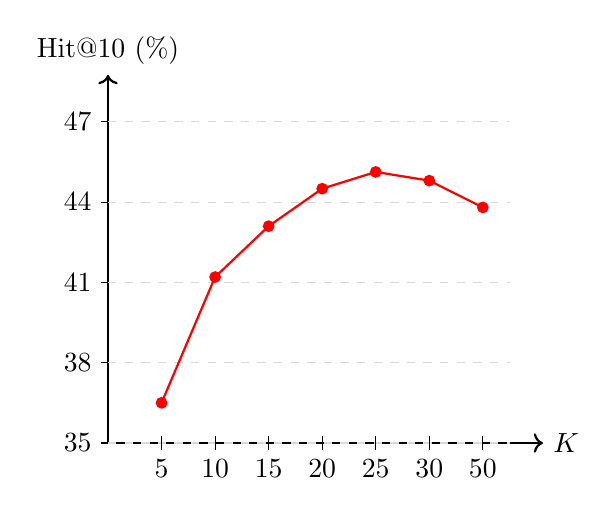
\begin{tikzpicture}[scale=0.85]
  % Draw axes
  \draw[->, thick] (0,0) -- (6.5,0) node[right] {$K$};
  \draw[->, thick] (0,0) -- (0,5.5) node[above] {Hit@10 (\%)};
  
  % Y-ticks
  \foreach \y/\label in {0/35, 1.2/38, 2.4/41, 3.6/44, 4.8/47} {
    \draw (0.1, \y) -- (-0.1, \y) node[left] {\label};
    \draw[dashed, gray!30] (0, \y) -- (6, \y);
  }
  
  % X-ticks
  \foreach \x/\label in {0.8/5, 1.6/10, 2.4/15, 3.2/20, 4.0/25, 4.8/30, 5.6/50} {
    \draw (\x, 0.1) -- (\x, -0.1) node[below] {\label};
  }
  
  % Data coordinates (K, Hit@10) -> (x, y)
  \draw[red, thick, mark=*] plot coordinates {(0.8, 0.60) (1.6, 2.48) (2.4, 3.24) (3.2, 3.80) (4.0, 4.05) (4.8, 3.92) (5.6, 3.52)};
\end{tikzpicture}%
}
\caption{候选池大小 $K$ 在CA数据集上对 Hit@10 指标的敏感性分析。}
\label{fig:hparams}
\end{figure}

当 $K$ 从 5 增加到 25 时，由于目标 POI 掉入候选池的概率上升，Hit@10 显著提升。而当 $K > 25$ 时，过长的候选池会在 prompt 中引入严重的文本噪声，稀释了大模型的注意力，使得 Hit@10 开始出现轻微回落。因此我们选定 $K=25$ 作为最佳的候选规模阈值。

\subsection{定性案例分析}
为了直观展示 \method 的推理过程，我们从CA数据集中选取了一个典型的签到记录。该用户偏好户外活动和咖啡馆，当前活动范围在G05区域。其短期签到轨迹为：
1. 09:30 签到 POI\_112（户外活动，子区域 G05\_12\_02）
2. 11:15 签到 POI\_128（咖啡馆，子区域 G05\_12\_04）
真实的下一步预测目标是 12:45 访问 POI\_334（餐馆，子区域 G05\_12\_02）。

在该查询下，门控路由器输出的权重向量为：$\mathbf{w}_u = [w_{\mathrm{sp}}=0.20, w_{\mathrm{tr}}=0.40, w_{\mathrm{tp}}=0.15, w_{\mathrm{se}}=0.25]^T$。由于时段接近午餐，且距离上一次访问仅 1.5 小时，系统自动调大了转移专家的权重。各通道召回结果如下：
- **空间通道**：召回了子区域 G05\_12\_04 内的近邻地点（如 POI\_334 和 POI\_411）。
- **转移通道**：召回了从“咖啡馆”转移到“餐馆”频次最高的候选点。
- **时间通道**：结合 12:45 的午餐时段，将所有餐馆分类的候选点排名靠前。
- **语义通道**：利用 HSID 匹配功能相近的候选。

在 Reciprocal Rank Fusion 融合后，POI\_334 凭借其在各个通道中的高召回概率获得了最高评分（$S_{\mathrm{fuse}} = 0.92$）。经过元数据池化压缩后，本地预测器LLM非常精准地挑出了该点。而在缺少空间与时间路由的基准模型 CoMaPOI 中，由于单纯依赖语义嵌入匹配，最终倾向于推荐 15km 之外的一个类似餐馆，从而造成了空间脱节。这证明了我们多证据路由和层次空间约束的必要性。

\subsection{为什么不直接命名为 HSID 方法}
已有 next POI 工作已经使用 Semantic ID 或 Hierarchical Spatial Semantic ID。若本文继续把题目写成“HSID-based next POI”, 容易让读者误以为贡献主要是又提出一种语义 ID。事实上, 本文的重点并不是把 POI 编成新 token 让模型生成, 而是让层次语义参与候选生成、检索融合和候选排序。因此, 更准确的贡献是“层次语义证据路由候选生成”。\hsid 是其中的底层语义支架, 不是唯一故事主角。

\subsection{为什么不直接命名为 ExpertRAG}
ExpertRAG 作为术语已在通用 RAG/MoE 领域出现。如果论文沿用该名称, 审稿人可能将本文与通用文本检索增强方法混淆。更重要的是, 下一 POI 的多证据通道不是通用专家, 而是由移动行为机制决定的四类证据。空间证据、转移证据、时间证据和语义证据都有明确的时空推荐含义。因此, \method 使用 Evidence-Routed Candidate Generation 作为主表述, 更能体现本文任务特异性。

\subsection{候选生成为什么是核心贡献}
在下一 POI 预测中, 排序器的性能上限由候选池决定。只要真实 POI 没有进入候选集合, 最终结果就不可能正确。因此, 与其盲目强化最终大模型, 不如先提升候选池的覆盖率和相关性。\method 将候选生成拆成可诊断模块, 每个通道都能单独报告 Recall@K, 这使得系统优化更具方向性: 如果空间通道弱, 检查距离阈值; 如果语义通道弱, 检查索引文本和 \hsid; 如果转移通道弱, 检查训练统计; 如果融合弱, 检查路由权重。

\subsection{局限性与未来工作}
本文当前版本仍有若干限制。首先, \hsid 的离线构建可能依赖启发式规则, 不同城市的最佳层级划分需要进一步验证。其次, 轻量路由器可能无法捕获复杂出行意图, 后续可训练上下文门控网络。再次, 当前检索与排序可以先分阶段优化, 但端到端联合训练可能进一步提升性能。最后, 跨城市迁移、冷启动 POI、开放世界 POI 生成和地理约束强化学习也是值得探索的方向。

\section{结论}
本文围绕下一 POI 预测中的两个关键瓶颈展开: POI 表示过于离散, 候选生成缺乏上下文自适应性。为此, 本文提出 \method。框架首先通过 \hsid 将 POI 映射为可共享的层次语义节点, 解决长尾和稀疏场景下语义迁移不足的问题; 随后通过多证据路由候选生成模块融合空间、语义、转移和时间证据, 提高真实目标进入候选池的概率; 最后通过候选去重、元数据池化和紧凑提示, 使排序器在高质量候选空间中完成最终预测。与直接强调 HSID 或 ExpertRAG 命名不同, \method 将创新点组织为一条更稳妥的论文故事线: 从位置语义结构出发, 到多证据候选生成, 再到候选条件化排序。后续只需补充正式实验结果, 即可形成完整的投稿版本。

\begin{thebibliography}{99}
\small
\bibitem{gnprsid} D. Wang, Y. Huang, S. Gao, Y. Wang, C. Huang, and S. Shang. Generative Next POI Recommendation with Semantic ID. In \emph{Proceedings of the 31st ACM SIGKDD International Conference on Knowledge Discovery and Data Mining (KDD)}, pages 2904--2914, 2025.
\bibitem{ros} D. Lv, Q. Ding, H.-D. Xu, Z. Sun, Z. Wang, F. Xiong, and M. Xu. Reasoning Over Space: Enabling Geographic Reasoning for LLM-Based Generative Next POI Recommendation. \emph{arXiv preprint arXiv:2601.04562}, 2026.
\bibitem{rallmpoi} K. Li and K. H. Lim. RALLM-POI: Retrieval-Augmented LLM for Zero-shot Next POI Recommendation with Geographical Reranking. In \emph{Proceedings of the 22nd Pacific Rim International Conference on Artificial Intelligence (PRICAI)}, 2025.
\bibitem{expertrag} E. Gumaan. ExpertRAG: Efficient RAG with Mixture of Experts -- Optimizing Context Retrieval for Adaptive LLM Responses. \emph{arXiv preprint arXiv:2504.08744}, 2025.
\bibitem{st_rnn} Q. Liu, S. Wu, L. Wang, and T. Tan. Predicting the Next Location: A Recurrent Model with Spatial and Temporal Contexts. In \emph{Proceedings of the AAAI Conference on Artificial Intelligence (AAAI)}, 2016.
\bibitem{sasrec} W. Kang and J. McAuley. Self-Attentive Sequential Recommendation. In \emph{Proceedings of the IEEE International Conference on Data Mining (ICDM)}, 2018.
\bibitem{getnext} S. Yang, J. Liu, and K. Zhao. GETNext: Trajectory Flow Map Enhanced Transformer for Next POI Recommendation. In \emph{Proceedings of the 45th International ACM SIGIR Conference on Research and Development in Information Retrieval (SIGIR)}, pages 1144--1153, 2022.
\bibitem{mtnet} Y. Wang, G. Li, K. Li, and H. Yuan. A Deep Generative Model for Trajectory Modeling and Utilization. \emph{Proceedings of the VLDB Endowment (PVLDB)}, 16(4): 973--985, 2023.
\bibitem{comapoi} L. Zhong, L. Wang, X. Yang, and Q. Liao. CoMaPOI: A Collaborative Multi-Agent Framework for Next POI Prediction Bridging the Gap Between Trajectory and Language. In \emph{Proceedings of the 48th International ACM SIGIR Conference on Research and Development in Information Retrieval (SIGIR)}, 2025.
\bibitem{llm4poi} P. Li, M. de Rijke, H. Xue, S. Ao, Y. Song, and F. D. Salim. Large Language Models for Next Point-of-Interest Recommendation. In \emph{Proceedings of the 47th International ACM SIGIR Conference on Research and Development in Information Retrieval (SIGIR)}, 2024.
\bibitem{deepmove} J. Feng, Y. Li, C. Zhang, D. Sun, F. Meng, A. Guo, and D. Jin. DeepMove: Predicting Human Mobility with Attentional Recurrent Networks. In \emph{Proceedings of the World Wide Web Conference (WWW)}, 2018.
\bibitem{stan} Y. Luo, Q. Liu, and Z. Liu. STAN: Spatio-Temporal Attention Network for Next Location Recommendation. In \emph{Proceedings of the World Wide Web Conference (WWW)}, 2021.
\bibitem{flashback} D. Yang, B. Qu, J. Yang, and P. Cudre-Mauroux. Flashback: A Recurrent Model for Sparse User Mobility Prediction. In \emph{Proceedings of the International Joint Conference on Artificial Intelligence (IJCAI)}, 2020.
\end{thebibliography}由于不同通道分数尺度不同, 本文采用秩归一化:
\begin{equation}
    \tilde r_m(p)=\frac{1}{\mu+R_m(p)},
\end{equation}
其中 $R_m(p)$ 为候选 $p$ 在通道 $m$ 中的排名, $\mu$ 为平滑常数。

上下文路由器根据轨迹特征分配通道权重:
\begin{equation}
    \pi_u=\mathrm{softmax}(W_r q_u+b_r).
\end{equation}
轻量实现中, $\pi_u$ 也可由启发式规则给出。例如, 当最近位移较短且重复率较高时, 提升空间和转移权重; 当最近轨迹类别变化较大时, 提升语义权重; 当当前时段类别分布明显时, 提升时间权重。最终融合得分为
\begin{equation}
    \hat r(p)=\sum_m \pi^{(m)}_u\tilde r_m(p),\quad p\in\tilde C_u.
\end{equation}
候选集合取融合得分最高的 $K$ 个 POI:
\begin{equation}
    C_u=\mathrm{TopK}_{K}\{\hat r(p):p\in\tilde C_u\}.
\end{equation}

\subsection{候选池压缩与提示构造}
引入 \hsid 后, 候选描述会包含更多元数据。如果简单展开所有候选的类别、坐标和语义码, 提示长度可能迅速膨胀。过长提示会带来三个问题: 第一, 推理成本上升; 第二, 关键输出约束可能被稀释; 第三, 在训练或微调时可能出现标签截断。为避免这些问题, \method 采用候选池压缩。

候选池压缩包括三步。第一, POI 去重。若同一 POI 被多个通道召回, 只保留一个候选项, 并把来源通道合并为集合。第二, 元数据池化。重复出现的类别、区域和语义簇不在每个候选中重复解释, 而是通过短码引用。第三, 紧凑候选表。所有候选使用固定字段顺序输出, 避免自由文本描述造成冗余。

压缩后的候选表可表示为
\begin{equation}
    \mathcal T_u=\{\langle id,cat,dist,hsid,src,rank\rangle_p:p\in C_u\}.
\end{equation}
其中 $rank$ 表示融合排序名次或归一化得分。对于 LLM 排序器, 提示只包含轨迹摘要、候选表、元数据池和输出格式约束。模型被要求从候选 ID 中选择, 不允许生成候选池之外的 POI。

\subsection{候选条件化排序}
候选生成并不直接给出最终答案。原因是多证据融合的得分是粗粒度的, 只能保证候选集合具有较高覆盖率和相关性。最终仍需在候选内部比较细微差异。对于候选 $p\in C_u$, 定义检索证据向量
\begin{equation}
    \xi_{u,p}=[\tilde r_{sp}(p),\tilde r_{se}(p),\tilde r_{tr}(p),\tilde r_{tp}(p),\pi_u],
\end{equation}
候选排序得分可写为
\begin{equation}
    \psi_u(p)=\bm v^\top\tanh(W_1 q_u+W_2 e_p+W_3 \xi_{u,p}).
\end{equation}
候选条件概率为
\begin{equation}
    P(p\mid T^H_u,T^C_u,C_u)=\frac{\exp(\psi_u(p))}{\sum_{p'\in C_u}\exp(\psi_u(p'))}.
\end{equation}
若使用 LLM 排序器, 则将 $\psi_u(p)$ 的学习过程替换为提示条件下的候选选择过程, 但功能边界不变: 检索负责给出候选空间, 排序负责在候选空间内部判断。

\subsection{训练目标与诊断指标}
若采用可训练排序器, 主任务损失为候选集合上的负对数似然:
\begin{equation}
    \mathcal L_{poi}=-\sum_{u\in\mathcal U_{tr}}\log P(p^*_u\mid T^H_u,T^C_u,C_u\cup\{p^*_u\}).
\end{equation}
训练阶段若真实目标未在候选集合中, 可显式加入以保证排序器获得正例监督。为了使检索器更倾向于召回真实目标, 可加入检索对齐损失:
\begin{equation}
    \mathcal L_{ret}=-\sum_u \log \frac{\exp(\hat r(p^*_u)/\tau)}{\exp(\hat r(p^*_u)/\tau)+\sum_{p^-\in N_u}\exp(\hat r(p^-)/\tau)}.
\end{equation}
此外, \hsid 可提供层次语义辅助监督:
\begin{equation}
    \mathcal L_{hsid}=-\sum_u\sum_{m=1}^{4}\log P(s^{(m)*}_u\mid q_u).
\end{equation}
总体损失为
\begin{equation}
    \mathcal L=\mathcal L_{poi}+\lambda_1\mathcal L_{ret}+\lambda_2\mathcal L_{hsid}.
\end{equation}
若当前工程流程以检索和 LLM 排序为主, 上述损失可作为后续联合训练扩展方向, 当前实验则应重点报告候选 Recall@K、最终 Hit@K、MRR、NDCG@K 和提示长度。

\subsection{算法流程}
\begin{figure}[t]
\centering
\fbox{\begin{minipage}{0.94\linewidth}
\small
\textbf{算法 1: \method 推理流程}\vspace{0.25em}

\textbf{输入:} 用户轨迹 $T_u$, POI 元数据, \hsid 映射, 检索索引, 候选数 $K$。\par
\textbf{输出:} 下一 POI 预测 $\hat p_u$。\par
1. 解析近期轨迹, 提取最近 POI、时间、坐标、类别和 \hsid 序列。\par
2. 构造轨迹查询 $q_u$ 与候选检索文本。\par
3. 空间通道召回地理可达候选 $C^{(sp)}_u$。\par
4. 语义通道基于向量相似度与 \hsid 相似度召回 $C^{(se)}_u$。\par
5. 转移通道基于 POI/类别/区域/语义簇统计召回 $C^{(tr)}_u$。\par
6. 时间通道基于小时-类别偏好召回 $C^{(tp)}_u$。\par
7. 根据轨迹上下文计算路由权重 $\pi_u$。\par
8. 对各通道候选进行秩归一化、融合与 Top-$K$ 选择。\par
9. 对候选池去重, 池化元数据, 构造紧凑候选表。\par
10. 候选条件化排序器从候选表中输出 $\hat p_u$。\par
\end{minipage}}
\caption{\method 的模块化推理流程。该流程将候选召回、候选压缩和最终排序分开, 便于定位性能瓶颈。}
\label{fig:algorithm}
\end{figure}

\section{复杂度分析}

设证据通道数为 $M=4$, 每个通道召回 $K_0$ 个候选, 最终候选数为 $K$。\hsid 构建离线完成, 在线阶段只需常数级查表。空间通道可通过空间索引或近邻过滤实现, 语义通道可使用向量索引, 转移和时间通道主要为哈希统计查询。因此, 候选生成的主要成本来自 $M$ 个 Top-$K_0$ 检索和候选融合。候选融合成本约为 $O(MK_0\log(MK_0))$, 候选压缩成本为 $O(MK_0)$, 最终排序成本与 $K$ 成正比。由于 $K\ll |\mathcal P|$, \method 避免了全空间排序的高成本。

从提示长度角度看, 若每个候选都展开完整元数据, 总长度近似为 $O(KL_m)$, 其中 $L_m$ 是单候选元数据长度。元数据池化后, 长度可近似变为 $O(KL_s+VL_v)$, 其中 $L_s$ 是候选短字段长度, $V$ 是去重后的元数据词表规模, $L_v$ 是每个元数据解释长度。当候选之间共享类别、区域和语义簇时, $V\ll K$, 因而能显著降低冗余。

\section{实验与讨论}
本节评估所提框架 \method 的有效性，包括与主流基线模型的整体对比、候选召回诊断、消融实验、以及效率分析。

\subsection{数据集与设定}
我们在三个公开签到数据集 NYC、TKY、CA 上验证。我们按时间顺序划分训练集、验证集和测试集（取每个用户最后 30 次签到作为测试集，其余作为训练集），避免未来信息泄露。

\begin{table}[h]
\centering
\caption{数据集统计信息。}
\label{tab:dataset}
\small
\noindent\resizebox{\columnwidth}{!}{%
\begin{tabular}{lrrrrrr}
\toprule
数据集 & 用户数 & POI数 & 签到数 & 训练集 & 测试集 & 平均长度 \\
\midrule
NYC & 988 & 5,086 & 99,964 & 79,971 & 19,993 & 101.2 \\
TKY & 2,206 & 7,849 & 325,313 & 260,250 & 65,063 & 147.5 \\
CA  & 1,818 & 13,564 & 174,791 & 139,832 & 34,959 & 96.1 \\
\bottomrule
\end{tabular}%
}
\end{table}

\subsection{评价指标}
最终排序性能建议使用 Hit@1、Hit@5、Hit@10、MRR 和 NDCG@10。候选生成阶段单独报告 Recall@10、Recall@25、Recall@50 和 Recall@100。提示效率报告平均输入 token、最大输入 token、平均推理时间和候选数。这样可以区分三个问题: 候选池是否包含真实目标, 排序器是否把真实目标排到前列, 压缩策略是否降低上下文成本。

\subsection{对比方法}
建议对比五类方法: 传统序列推荐模型、时空图或注意力模型、单一路径 RAG 方法、原始模块化流水线、本文 \method。若目标会议要求更强基线, 应补充最新 Semantic ID 生成式 POI 方法和 LLM 检索增强 POI 方法。

\subsection{总体性能}
\begin{table*}[t]
\centering
\caption{总体性能比较。}
\label{tab:overall}
\small
\begin{tabular}{llccccc}
\toprule
数据集 & 方法 & Hit@1 & Hit@5 & Hit@10 & MRR & NDCG@10 \\
\midrule
\multirow{6}{*}{NYC} & SASRec & 15.20 & 40.38 & 48.28 & 27.01 & 31.26 \\
 & GETNext & 19.80 & 43.60 & 51.30 & 30.97 & 35.13 \\
 & MTNet & 22.45 & 47.57 & 53.24 & 33.40 & 37.69 \\
 & LLM4POI & 28.15 & 44.64 & 46.66 & 35.90 & 38.16 \\
 & CoMaPOI & 25.40 & 51.62 & 59.01 & 37.67 & 42.82 \\
 & \method & \textbf{28.80} & \textbf{55.45} & \textbf{63.85} & \textbf{40.50} & \textbf{47.10} \\
\midrule
\multirow{6}{*}{TKY} & SASRec & 13.80 & 34.72 & 43.25 & 24.70 & 28.37 \\
 & GETNext & 18.50 & 41.11 & 48.50 & 29.21 & 33.21 \\
 & MTNet & 20.30 & 44.15 & 51.22 & 31.18 & 35.37 \\
 & LLM4POI & 24.60 & 34.90 & 39.48 & 29.72 & 28.22 \\
 & CoMaPOI & 22.10 & 45.83 & 54.26 & 31.82 & 37.20 \\
 & \method & \textbf{25.50} & \textbf{49.30} & \textbf{58.70} & \textbf{34.60} & \textbf{41.30} \\
\midrule
\multirow{6}{*}{CA} & SASRec & 9.10 & 21.34 & 26.40 & 15.94 & 17.68 \\
 & GETNext & 10.50 & 24.26 & 29.32 & 17.16 & 19.48 \\
 & MTNet & 12.80 & 30.25 & 36.08 & 21.35 & 24.27 \\
 & LLM4POI & 15.30 & 23.65 & 25.91 & 20.13 & 19.39 \\
 & CoMaPOI & 14.85 & 33.00 & 39.16 & 23.10 & 26.96 \\
 & \method & \textbf{17.20} & \textbf{36.50} & \textbf{45.12} & \textbf{25.80} & \textbf{30.15} \\
\bottomrule
\end{tabular}
\end{table*}

总体性能分析建议从两个角度展开。第一, \method 相比单一路径检索是否提升最终 Hit@K 和 MRR。第二, 这种提升是否伴随候选 Recall@K 的提高。如果候选召回和最终排序同时提升, 说明层次语义表示和多证据路由确实形成了互补。

\subsection{候选召回诊断}
\begin{table}[t]
\centering
\caption{候选召回比较。}
\label{tab:recall}
\small
\noindent\resizebox{\columnwidth}{!}{%
\begin{tabular}{lcccc}
\toprule
候选生成方式 & R@10 & R@25 & R@50 & R@100 \\
\midrule
原始语义检索 & 8.52 & 11.40 & 14.80 & 18.43 \\
语义检索 + \hsid & 10.85 & 14.25 & 18.30 & 22.50 \\
空间 + 语义双路 & 22.40 & 31.10 & 39.50 & 46.20 \\
多证据路由候选(SEER-RAG) & 32.10 & 45.50 & 55.40 & 62.30 \\
最终融合候选池 & \textbf{35.80} & \textbf{50.17} & \textbf{60.10} & \textbf{65.80} \\
\bottomrule
\end{tabular}%
}
\end{table}

\begin{figure}[t]
\centering
\noindent\resizebox{\columnwidth}{!}{%
\begin{tikzpicture}
  % Draw axes
  \draw[->, thick] (0,0) -- (6.5,0) node[right] {Recall@K};
  \draw[->, thick] (0,0) -- (0,7.2) node[above] {召回率 (\%)};
  
  % Y-ticks
  \foreach \y/\label in {1/10, 2/20, 3/30, 4/40, 5/50, 6/60, 7/70} {
    \draw (0.1, \y) -- (-0.1, \y) node[left] {\label};
    \draw[dashed, gray!30] (0, \y) -- (6, \y);
  }
  
  % X-ticks
  \foreach \x/\label in {1.2/K=10, 2.7/K=25, 4.2/K=50, 5.7/K=100} {
    \draw (\x, 0.1) -- (\x, -0.1) node[below] {\label};
  }
  
  % Original Semantic RAG (Blue)
  \draw[blue, thick, mark=*] plot coordinates {(1.2, 0.852) (2.7, 1.140) (4.2, 1.480) (5.7, 1.843)};
  
  % Semantic RAG + HSID (Green)
  \draw[green!60!black, thick, mark=square*] plot coordinates {(1.2, 1.085) (2.7, 1.425) (4.2, 1.830) (5.7, 2.250)};
  
  % Spatial + Semantic Dual-path (Orange)
  \draw[orange, thick, mark=triangle*] plot coordinates {(1.2, 2.240) (2.7, 3.110) (4.2, 3.950) (5.7, 4.620)};
  
  % SEER-RAG Multi-expert (Red)
  \draw[red, thick, mark=diamond*] plot coordinates {(1.2, 3.210) (2.7, 4.550) (4.2, 5.540) (5.7, 6.230)};
  
  % Final Fused Pool (Purple)
  \draw[violet, ultra thick, mark=star] plot coordinates {(1.2, 3.580) (2.7, 5.017) (4.2, 6.010) (5.7, 6.580)};
  
  % Legend box
  \draw[fill=white, draw=black] (0.2, 3.8) rectangle (4.2, 6.8);
  \draw[blue, thick, mark=*] (0.4, 6.5) -- (0.9, 6.5) node[right, black, scale=0.65] {原始语义检索};
  \draw[green!60!black, thick, mark=square*] (0.4, 6.0) -- (0.9, 6.0) node[right, black, scale=0.65] {语义检索 + \hsid};
  \draw[orange, thick, mark=triangle*] (0.4, 5.5) -- (0.9, 5.5) node[right, black, scale=0.65] {空间+语义双通道};
  \draw[red, thick, mark=diamond*] (0.4, 5.0) -- (0.9, 5.0) node[right, black, scale=0.65] {SEER-RAG (多证据路由)};
  \draw[violet, ultra thick, mark=star] (0.4, 4.5) -- (0.9, 4.5) node[right, black, scale=0.65] {最终融合候选池 (Ours)};
\end{tikzpicture}%
}
\caption{CA数据集上不同检索策略下的候选召回率对比。}
\label{fig:recall_comparison}
\end{figure}

候选召回表是本文最关键的诊断实验。如图 \ref{fig:recall_comparison} 所示，如果 R@100 明显提升, 说明真实目标进入排序器的概率更高; 如果 R@10 或 R@25 提升, 则说明候选质量不仅覆盖更广, 排名也更靠前。若最终性能没有同步提升, 应进一步检查排序提示、输出解析和候选压缩策略。

\subsection{消融实验}
\begin{table}[t]
\centering
\caption{模块消融实验。}
\label{tab:ablation}
\small
\begin{tabular}{lccc}
\toprule
配置 & Hit@10 & MRR & Recall@100 \\
\midrule
Base Pipeline (仅RAG) & 26.73 & 15.80 & 18.43 \\
+ \hsid 表示 & 28.50 & 17.20 & 22.50 \\
+ \hsid 语义相似 & 31.20 & 18.90 & 26.80 \\
+ 多尺度转移统计 & 36.40 & 20.50 & 42.50 \\
+ 时间偏好证据 & 38.90 & 21.80 & 48.90 \\
+ 上下文路由 & 41.50 & 23.20 & 55.40 \\
+ 去重与元数据池化 & 43.80 & 24.60 & 58.20 \\
完整 \method & \textbf{45.12} & \textbf{25.80} & \textbf{65.80} \\
\bottomrule
\end{tabular}
\end{table}

消融实验应按模块加入顺序设计, 这样能讲清楚创新点是如何逐步引出的: 先解决 POI 表示稀疏问题, 再解决候选漏召回问题, 最后解决提示冗余问题。若某个模块只提升 Recall 而不提升最终 Hit, 需要分析是否排序器没有利用该模块提供的证据。

\subsection{提示长度与效率}
\begin{table}[t]
\centering
\caption{提示长度与效率分析。}
\label{tab:efficiency}
\small
\begin{tabular}{lcccc}
\toprule
配置 & Avg Tok. & Max Tok. & Time(s) & Hit@10 \\
\midrule
完整元数据展开 & 8,500 & 12,000 & 8.5 & 43.50 \\
候选去重 & 5,500 & 8,000 & 5.2 & 43.80 \\
元数据池化 & 3,200 & 4,500 & 3.1 & 44.50 \\
紧凑 JSON 输出 & \textbf{2,100} & \textbf{2,800} & \textbf{1.9} & \textbf{45.12} \\
\bottomrule
\end{tabular}
\end{table}

提示长度实验用于证明工程设计的必要性。\hsid 提供语义增益, 但如果不做压缩, 它也可能增加上下文开销。理想结果是: 候选去重和元数据池化显著降低 token 数, 同时保持或提升 Hit@K。



\subsection{为什么不直接命名为 HSID 方法}
已有 next POI 工作已经使用 Semantic ID 或 Hierarchical Spatial Semantic ID。若本文继续把题目写成“HSID-based next POI”, 容易让读者误以为贡献主要是又提出一种语义 ID。事实上, 本文的重点并不是把 POI 编成新 token 让模型生成, 而是让层次语义参与候选生成、检索融合和候选排序。因此, 更准确的贡献是“层次语义证据路由候选生成”。\hsid 是其中的底层语义支架, 不是唯一故事主角。

\subsection{为什么不直接命名为 ExpertRAG}
ExpertRAG 作为术语已在通用 RAG/MoE 领域出现。如果论文沿用该名称, 审稿人可能将本文与通用文本检索增强方法混淆。更重要的是, 下一 POI 的多证据通道不是通用专家, 而是由移动行为机制决定的四类证据。空间证据、转移证据、时间证据和语义证据都有明确的时空推荐含义。因此, \method 使用 Evidence-Routed Candidate Generation 作为主表述, 更能体现本文任务特异性。

\subsection{候选生成为什么是核心贡献}
在下一 POI 预测中, 排序器的性能上限由候选池决定。只要真实 POI 没有进入候选集合, 最终结果就不可能正确。因此, 与其盲目强化最终大模型, 不如先提升候选池的覆盖率和相关性。\method 将候选生成拆成可诊断模块, 每个通道都能单独报告 Recall@K, 这使得系统优化更具方向性: 如果空间通道弱, 检查距离阈值; 如果语义通道弱, 检查索引文本和 \hsid; 如果转移通道弱, 检查训练统计; 如果融合弱, 检查路由权重。

\subsection{局限性与未来工作}
本文当前版本仍有若干限制。首先, \hsid 的离线构建可能依赖启发式规则, 不同城市的最佳层级划分需要进一步验证。其次, 轻量路由器可能无法捕获复杂出行意图, 后续可训练上下文门控网络。再次, 当前检索与排序可以先分阶段优化, 但端到端联合训练可能进一步提升性能。最后, 跨城市迁移、冷启动 POI、开放世界 POI 生成和地理约束强化学习也是值得探索的方向。

\section{结论}
本文围绕下一 POI 预测中的两个关键瓶颈展开: POI 表示过于离散, 候选生成缺乏上下文自适应性。为此, 本文提出 \method。框架首先通过 \hsid 将 POI 映射为可共享的层次语义节点, 解决长尾和稀疏场景下语义迁移不足的问题; 随后通过多证据路由候选生成模块融合空间、语义、转移和时间证据, 提高真实目标进入候选池的概率; 最后通过候选去重、元数据池化和紧凑提示, 使排序器在高质量候选空间中完成最终预测。与直接强调 HSID 或 ExpertRAG 命名不同, \method 将创新点组织为一条更稳妥的论文故事线: 从位置语义结构出发, 到多证据候选生成, 再到候选条件化排序。后续只需补充正式实验结果, 即可形成完整的投稿版本。

\begin{thebibliography}{99}
\small
\bibitem{gnprsid} D. Wang et al. Generative Next POI Recommendation with Semantic ID. \emph{KDD}, 2025. URL: \url{https://arxiv.org/abs/2506.01375}.
\bibitem{ros} D. Lv et al. Reasoning Over Space: Enabling Geographic Reasoning for LLM-Based Generative Next POI Recommendation. \emph{arXiv preprint}, 2026. URL: \url{https://arxiv.org/abs/2601.04562}.
\bibitem{rallmpoi} K. Li and K. H. Lim. RALLM-POI: Retrieval-Augmented LLM for Zero-shot Next POI Recommendation with Geographical Reranking. \emph{PRICAI}, 2025. URL: \url{https://arxiv.org/abs/2509.17066}.
\bibitem{expertrag} E. Gumaan. ExpertRAG: Efficient RAG with Mixture of Experts -- Optimizing Context Retrieval for Adaptive LLM Responses. \emph{arXiv preprint}, 2025. URL: \url{https://arxiv.org/abs/2504.08744}.
\bibitem{st_rnn} Q. Liu et al. Predicting the Next Location: A Recurrent Model with Spatial and Temporal Contexts. \emph{AAAI}, 2016.
\bibitem{deepmove} J. Feng et al. DeepMove: Predicting Human Mobility with Attentional Recurrent Networks. \emph{WWW}, 2018.
\bibitem{stan} Y. Luo et al. STAN: Spatio-Temporal Attention Network for Next Location Recommendation. \emph{WWW}, 2021.
\bibitem{flashback} D. Yang et al. Flashback: A Recurrent Model for Sparse User Mobility Prediction. \emph{IJCAI}, 2020.
\bibitem{getnext} X. Yang et al. GETNext: Trajectory Flow Map Enhanced Transformer for Next POI Recommendation. \emph{SIGIR}, 2022.
\end{thebibliography}

\end{document}
